%%%%%%%%%%%%%%%%%%%%%%%%%%%%%%%
\section{Traffic Trends: Overall}\label{sec:traffic}
%%%%%%%%%%%%%%%%%%%%%%%%%%%%%%%

Before delving into the details of the collaborating opportunities for content
providers and infrastructures we embark on giving an overview of typical
characteristics of Internet traffic.  We start by summarizing previous studies
on how Internet traffic looks like. We consider four aspects: \first The
composition of the application mix, \second popular content-types, \third the
distribution of traffic over the course of a day, and \fourth the distribution
of connection sizes.

\subsection{Application Mix}\label{sec:related:appmix}


One constant in the Internet during the last 10 years has been its steady
growth by more than 50\perc each year~\cite{andrew03growth,telegeography2008}.
Initially, protocols such as FTP, SMTP, and NNTP were popular. Then, in about
1994, HTTP entered into the picture. Until 2000, P2P protocols such as Napster
and Gnutella became popular but were later overtaken by eDonkey and BitTorrent.
However, the traffic mix has undergone substantial changes. Therefore, we now
revisit previously reported results regarding the application mix of Internet
traffic. For this purpose we rely on various studies that report on the
application mix between 2007 and 2009 from different vantage points:

\begin{itemize*}

\item The study by Maier \etal~\cite{OnDominantCharacteristics2009}, which is
based on a subset of the traces studied in Section~\ref{sec:impact}. It was
presented at IMC\,'09.

\item Two studies by ipoque~\cite{ipoque09}, which report on different regions
in the world (Germany and Middle East).  These studies are available for
download after registration via a Web form.

\item The Arbor report~\cite{arbor} on the ATLAS Internet Observatory presented
at a recent NANOG\footnote{NANOG is the North American Network Operators
Group.} meeting.

\item The Sandvine report on ``Global Broadband Phenomena''~\cite{sandvine}.

\end{itemize*}

In order to compare the results we have to summarize and unify the traffic
categories as each study uses their own nomenclature (see
Figure~\ref{fig:related:appmix}). For this purpose we use the following seven
categories:

\begin{description}

\item [Web.] All HTTP traffic including One-Click-Hosters (OCHs or Direct
Download Providers) but excluding video and audio streaming over HTTP (\ie
Flash-Video).

\item [Streaming.] All types of streaming in the Internet including streaming
over HTTP, RTP, RTSP, RTMP, ShoutCast, etc.

\item [Usenet.] The article reading and posting system that evolved from UUnet
and which uses NNTP as protocol.

\item [BitTorrent/P2P.] The popular P2P-protocol BitTorrent and all other P2P
traffic that is not eDonkey. Note, that the P2P traffic that is not BitTorrent
or eDonkey only adds a tiny fraction.  Moreover, this category represents all
P2P traffic if the study no further subdivides P2P traffic. This is the case
for Arbor~\cite{arbor} and Sandvine~\cite{sandvine}. Note as well, that the
Arbor study~\cite{arbor} reports a table with traffic shares, stating 0.95\perc
for P2P. This table is annotated with the comment that P2P is more likely to
account for 18\perc based on payload inspection of a limited data subset.

\item [eDonkey.] Another P2P protocol, if reported.

\item [Other/known.] Other identified traffic, for details we refer to the
corresponding studies.

\item [Unclassified.] Traffic that has not been classified. Note, that the
Sandvine~\cite{sandvine} study does not mention unclassified traffic, which
either implies a minute fraction or that it is missing in the plot.

\end{description}

\begin{figure}[tbp]
\centering
\includegraphics[width=0.95\linewidth]{figures/appmix.eps}
\renewcommand{\capname}{Barplot of the application mix in the
Internet\xspace}
\caption[\capname]{\capname (unified categories) for different years,
different regions according to several
sources~\cite{OnDominantCharacteristics2009,ipoque09,arbor,sandvine}.
\capcomment (BitTorrent/P2P contains all P2P except eDonkey.)}
\label{fig:related:appmix}
\end{figure}

Looking at these statistics we find that all studies report a significant
fraction of Web traffic. Indeed, Web is dominant ($>$ 50\perc) in most studies,
followed by P2P and streaming. It is noteworthy that Usenet is responsible for
a non-negligible fraction in several studies. This is surprising and a good
example for the importance of revisiting the application mix periodically in
order to identify new trends.

In terms of P2P protocol distribution Figure~\ref{fig:related:appmix} shows
that BitTorrent is dominating and the shares of eDonkey are decreasing.  Thus,
we note that the results of Plissonneau \etal~\cite{plissonneau05} who observed
91\perc of the P2P traffic is due to eDonkey in 2004 are no longer applicable.
Indeed, the popularity among P2P protocols swapped in favor of BitTorrent. We
can also see a general trend: P2P is declining according to all studies. This
is also supported by the results of Anderson~\cite{p2pdrops}. He points out
that this decline comes with an increase in video streaming. Moreover, most of
the studies pointed out that currently One-Click-Hoster (\eg Rapidshare or
MegaUpload) are as important for file-sharing as P2P systems.

Of course there are also trends that do not impact the application mix, for
example Online Social Networks (OSNs) such as Facebook. This is due to the fact
that OSNs use HTTP and they do not transport large videos, but profile
elements. Nevertheless, OSNs are not unimportant given the huge number of OSN
users world-wide.


\subsection{Content-types in the Internet}\label{sec:related:ctypes}

Next, we turn to the popularity of content-types in the Internet. Again, we
leverage several data sources, namely Maier
\etal~\cite{OnDominantCharacteristics2009}, ipoque~\cite{ipoque09}, and Erman
\etal~\cite{network-caching}. Once more we unify the categories and present
results for contents transferred via BitTorrent, eDonkey, and HTTP. See
Figure~\ref{fig:related:ctypes} for a summary.

\begin{figure}[tbp]
\centering
\includegraphics[width=0.95\linewidth]{figures/ctypes.eps}
\renewcommand{\capname}{Barplot of content-type popularity in the
Internet\xspace}
\caption[\capname]{\capname (unified categories) for
different protocols, different regions according to several
sources~\cite{OnDominantCharacteristics2009,ipoque09,network-caching}.}
\label{fig:related:ctypes}
\end{figure}

We see that videos are the most popular content in P2P systems (BitTorrent and
eDonkey). Even in HTTP videos account for more traffic than any other category.
Although HTTP was designed to transfer Web pages (text, \eg HTML, XML, CSS,
JavaScript, and image files) these contribute less than a third of the total
HTTP volume.

Overall, a significant fraction of software and archives is noticeable.
According to Maier \etal~\cite{OnDominantCharacteristics2009} almost all videos
are in flash-video format and are served by video portals such as YouTube.
Similarly, almost all archives are served by One-Click-Hosters. This is
confirmed by the results of Erman \etal~\cite{network-caching}.

Shifts in the popularity of content-types can be another indicator of new
trends. For example, there have been almost no flash-videos before the
breakthrough of YouTube.



\subsection{Time-of-day Effects}\label{sec:related:tod}

In order to understand when people are active in the Internet we show
time-of-day usage plots of link utilization from Maier
\etal~\cite{OnDominantCharacteristics2009} in
Figure~\ref{fig:related:tod-maier}, and aggregated traffic volume
Sandvine~\cite{sandvine} in Figure~\ref{fig:related:tod-sandvine}.

\begin{figure}[tbp]
\centering
\includegraphics[angle=-90,width=0.85\linewidth]{figures/maier-tod.eps}
\renewcommand{\capname}{Timeseries of link utilization from Maier \etal}
\caption[\capname]{\capname~\cite{OnDominantCharacteristics2009}}
\label{fig:related:tod-maier}
\end{figure}


\begin{figure}[tbp]
\centering
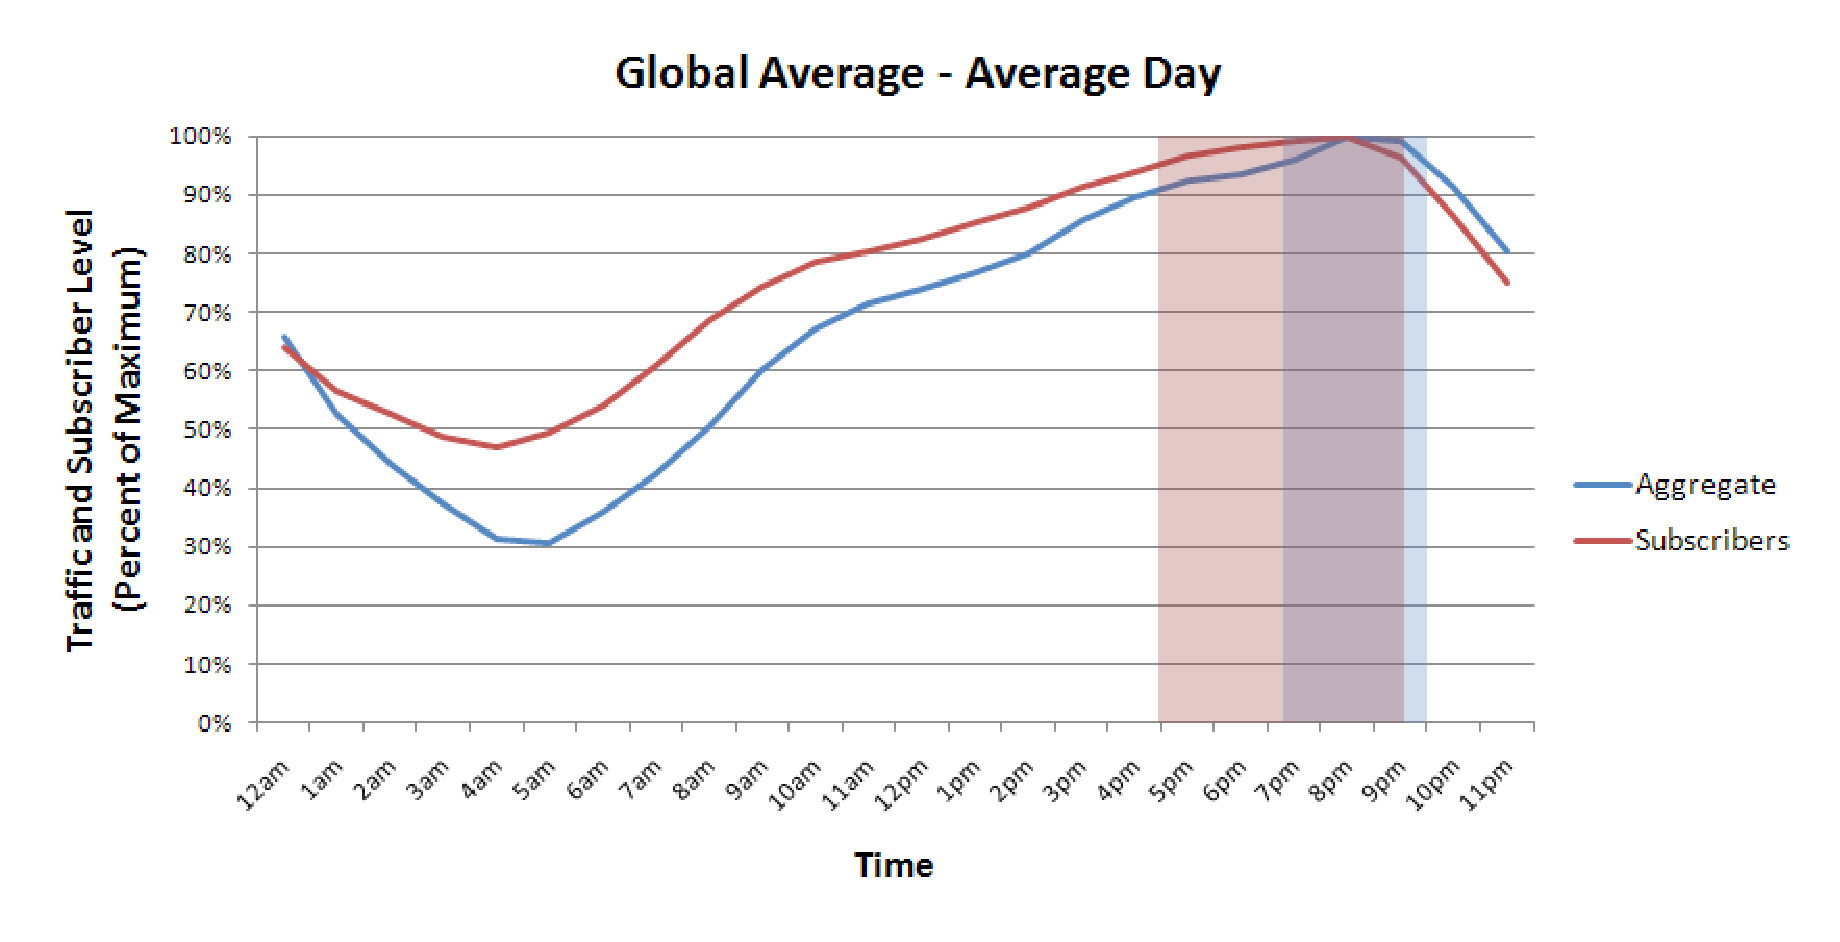
\includegraphics[width=0.85\linewidth]{figures/sandvine-tod.eps}
\renewcommand{\capname}{Timeseries of traffic volume from Sandvine\xspace}
\caption[\capname]{\capname~\cite{sandvine}}
\label{fig:related:tod-sandvine}
\end{figure}

In general, we observe a peak utilization at prime-time around 8\,pm and a
daily low between 2\,am and 4\,am. As the data sets of all these studies are
primarily collected from residential networks, it not surprising that they all
show similar characteristics. The peak usage in the evening hours can easily be
explained by the fact that people are usually not at home during business
hours. Rising demands just before lunch and in the afternoon may be due to
children returning home from school.

